% SECTION : graphs {{{
\clearpage
\section{Graphs}
\label{sec:graphs}
\parindent=0em



% sin(x)  {{{

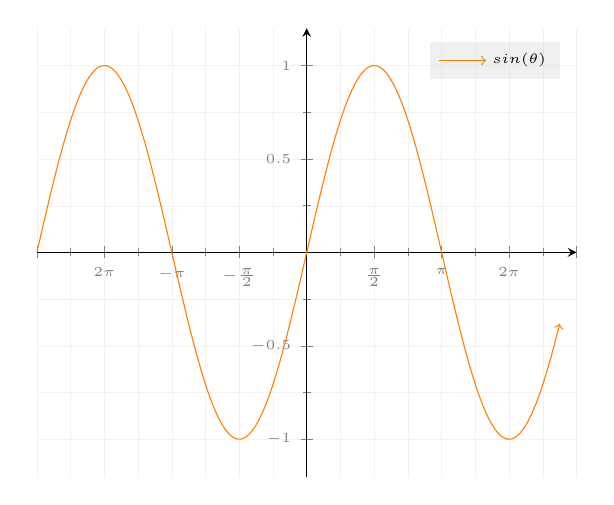
\begin{tikzpicture}
% axis settings {{{

\begin{axis}[
%	title          = graph_name,
	axis x line    = middle, % x-axis position
	axis y line    = middle, % y-axis position
	minor tick num = 1,      % num axis ticks
	grid           = both,
	grid style     =
	{
		line width = .1pt,
		draw       = gray!10
	},
	xmax      = 8,
	xmin      = -8,
	ymax      = 1.2,
	ymin      = -1.2,
	tick label style = {
		font  = \tiny,
		color = gray
	},
%	extra x ticks={3,1},
%	extra x tick labels={$\leftarrow$,$\rightarrow$},
%	extra y ticks={3,1},
%	extra y tick labels={$\leftarrow$,$\rightarrow$},
    xticklabels={ , , \( 2\pi \) , \( -\pi \) , \( -\frac{\pi}{2}  \) ,0, \( \frac{\pi}{2}  \), \( \pi \), \( 2\pi \)},
	legend style =
	{
		draw         = none, % remove legend bounding box
		font         = \tiny,
		legend pos   = north east,
		cells        = {anchor = west},
		fill         = gray!30,
		fill opacity = 0.4,
		text opacity = 1
	},
	%xlabel       = {$\scriptstyle rad$},
	%ylabel       = {$\scriptstyle y$},
	xlabel style =
	{
		at     = {(ticklabel* cs:1)},
%		anchor = north west
	},
	ylabel style =
	{
		at     = {(ticklabel* cs:1)},
%		anchor = south west
	}
]
% }}}
\coordinate (O) at (0,0);

\addplot [
	domain=-8:7.5,
	samples=300,
	orange,
	->
]
{sin(deg(\x*pi/4))};
\addlegendentry{$sin(\theta)$};


\end{axis}
\end{tikzpicture}

% }}}
% cos(x)  {{{

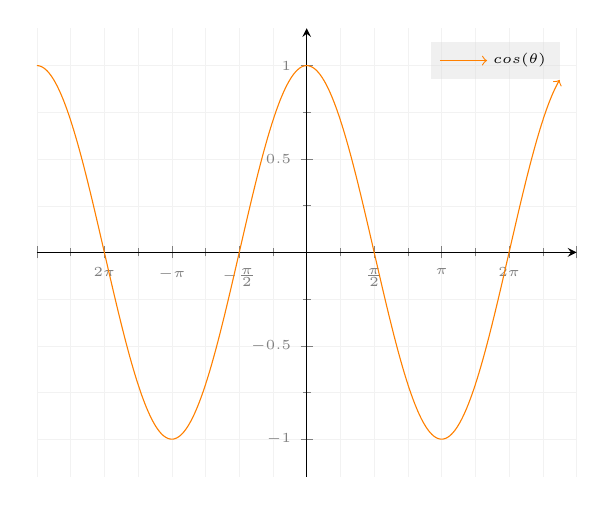
\begin{tikzpicture}
% axis settings {{{

\begin{axis}[
%	title          = graph_name,
	axis x line    = middle, % x-axis position
	axis y line    = middle, % y-axis position
	minor tick num = 1,      % num axis ticks
	grid           = both,
	grid style     =
	{
		line width = .1pt,
		draw       = gray!10
	},
	xmax      = 8,
	xmin      = -8,
	ymax      = 1.2,
	ymin      = -1.2,
	tick label style = {
		font  = \tiny,
		color = gray
	},
%	extra x ticks={3,1},
%	extra x tick labels={$\leftarrow$,$\rightarrow$},
%	extra y ticks={3,1},
%	extra y tick labels={$\leftarrow$,$\rightarrow$},
    xticklabels={ , , \( 2\pi \) , \( -\pi \) , \( -\frac{\pi}{2}  \) ,0, \( \frac{\pi}{2}  \), \( \pi \), \( 2\pi \)},
	legend style =
	{
		draw         = none, % remove legend bounding box
		font         = \tiny,
		legend pos   = north east,
		cells        = {anchor = west},
		fill         = gray!30,
		fill opacity = 0.4,
		text opacity = 1
	},
	%xlabel       = {$\scriptstyle rad$},
	%ylabel       = {$\scriptstyle y$},
	xlabel style =
	{
		at     = {(ticklabel* cs:1)},
%		anchor = north west
	},
	ylabel style =
	{
		at     = {(ticklabel* cs:1)},
%		anchor = south west
	}
]
% }}}
\coordinate (O) at (0,0);

\addplot [
	domain=-8:7.5,
	samples=300,
	orange,
	->
]
{cos(deg(\x*pi/4))};
\addlegendentry{$cos(\theta)$};


\end{axis}
\end{tikzpicture}

% }}}

% ln(x)  {{{

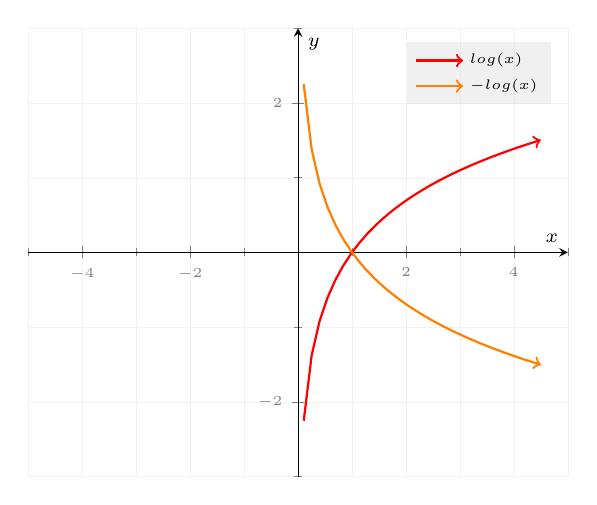
\begin{tikzpicture}
% axis settings {{{

\begin{axis}[
%	title          = graph_name,
	axis x line    = middle, % x-axis position
	axis y line    = middle, % y-axis position
	minor tick num = 1,      % num axis ticks
	grid           = both,
	grid style     =
	{
		line width = .1pt,
		draw       = gray!10
	},
	xmax      = 5,
	xmin      = -5,
	ymax      = 3,
	ymin      = -3,
	tick label style = {
		font  = \tiny,
		color = gray
	},
%	extra x ticks={3,1},
%	extra x tick labels={$\leftarrow$,$\rightarrow$},
%	extra y ticks={3,1},
%	extra y tick labels={$\leftarrow$,$\rightarrow$},
	legend style =
	{
		draw         = none, % remove legend bounding box
		font         = \tiny,
		legend pos   = north east,
		cells        = {anchor = west},
		fill         = gray!30,
		fill opacity = 0.4,
		text opacity = 1
	},
	xlabel       = {$\scriptstyle x$},
	ylabel       = {$\scriptstyle y$},
	xlabel style =
	{
		at     = {(ticklabel* cs:1)},
%		anchor = north west
	},
	ylabel style=
	{
		at     = {(ticklabel* cs:1)},
%		anchor = south west
	}
]
% }}}
\coordinate (O) at (0,0);

\addplot [
	domain=-10:4.5,
	samples=100,
	thick,
	red,
	->
]
{ln(x)};
\addlegendentry{$log(x)$};

\addplot [
	domain=-10:4.5,
	samples=100,
	thick,
	orange,
	->
]
{-ln(x)};
\addlegendentry{$-log(x)$};
\end{axis}
\end{tikzpicture}

% }}}
% ln(-x)  {{{

\begin{tikzpicture}
% axis settings {{{

\begin{axis}[
%	title          = graph_name,
	axis x line    = middle, % x-axis position
	axis y line    = middle, % y-axis position
	minor tick num = 1,      % num axis ticks
	grid           = none,
	grid style     =
	{
		line width = .1pt,
		draw       = gray!30
	},
	xmax      = 5,
	xmin      = -5,
	ymax      = 3,
	ymin      = -3,
	tick label style = {
		font  = \tiny,
		color = gray!30
	},
%	extra x ticks={3,1},
%	extra x tick labels={$\leftarrow$,$\rightarrow$},
%	extra y ticks={3,1},
%	extra y tick labels={$\leftarrow$,$\rightarrow$},
	legend style =
	{
		draw         = none, % remove legend bounding box
		font         = \tiny,
		legend pos   = outer north east,
		cells        = {anchor = west},
		fill         = gray,
		fill opacity = 0.4,
		text opacity = 1
	},
	xlabel       = {$\scriptstyle x$},
	ylabel       = {$\scriptstyle y$},
	xlabel style =
	{
		at     = {(ticklabel* cs:1)},
%		anchor = north west
	},
	ylabel style=
	{
		at     = {(ticklabel* cs:1)},
%		anchor = south west
	}
]
% }}}

\coordinate (O) at (0,0);

\addplot [
	domain=-10:10,
	samples=100,
	thick,
	orange,
	->
]
{ln(-x)};
%\addlegendentry{$\frac{1}{1+e^{-x}}$};

\end{axis}
\end{tikzpicture}

% }}}

% e^x  {{{

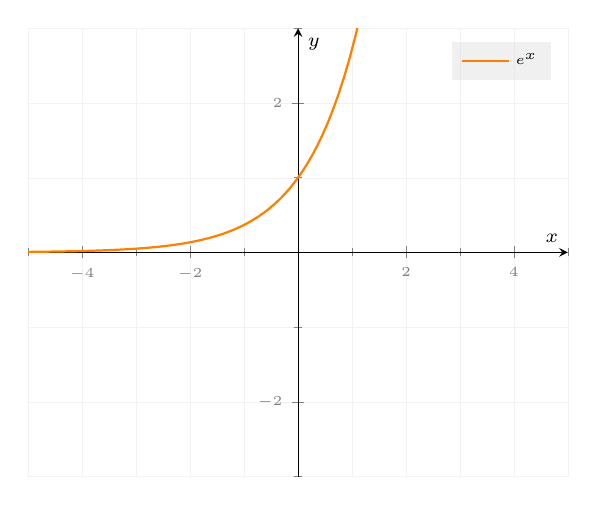
\begin{tikzpicture}
% axis settings {{{

\begin{axis}[
%	title          = graph_name,
	axis x line    = middle, % x-axis position
	axis y line    = middle, % y-axis position
	minor tick num = 1,      % num axis ticks
	grid           = both,
	grid style     =
	{
		line width = .1pt,
		draw       = gray!10
	},
	xmax      = 5,
	xmin      = -5,
	ymax      = 3,
	ymin      = -3,
	tick label style = {
		font  = \tiny,
		color = gray
	},
%	extra x ticks={3,1},
%	extra x tick labels={$\leftarrow$,$\rightarrow$},
%	extra y ticks={3,1},
%	extra y tick labels={$\leftarrow$,$\rightarrow$},
	legend style =
	{
		draw         = none, % remove legend bounding box
		font         = \tiny,
		legend pos   = north east,
		cells        = {anchor = west},
		fill         = gray!30,
		fill opacity = 0.4,
		text opacity = 1
	},
	xlabel       = {$\scriptstyle x$},
	ylabel       = {$\scriptstyle y$},
	xlabel style =
	{
		at     = {(ticklabel* cs:1)},
%		anchor = north west
	},
	ylabel style=
	{
		at     = {(ticklabel* cs:1)},
%		anchor = south west
	}
]
% }}}
\coordinate (O) at (0,0);

\addplot [
	domain=-5:5,
	no marks,
	samples=100,
	thick,
	orange
]
{exp(x)};
\addlegendentry{$e^x$};

\end{axis}
\end{tikzpicture}

% }}}
% sqrt(x)  {{{

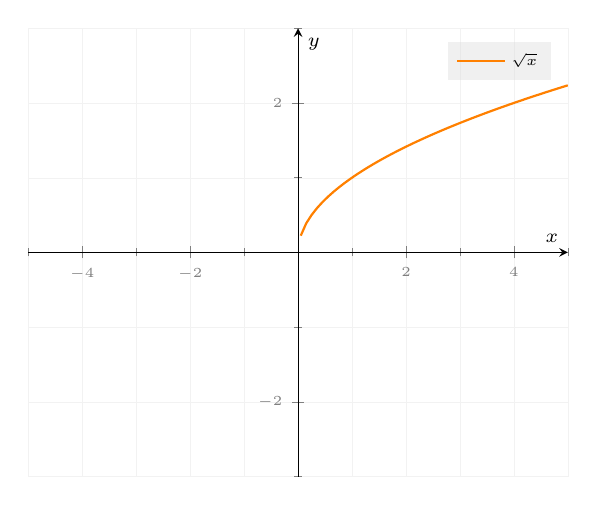
\begin{tikzpicture}
% axis settings {{{

\begin{axis}[
%	title          = graph_name,
	axis x line    = middle, % x-axis position
	axis y line    = middle, % y-axis position
	minor tick num = 1,      % num axis ticks
	grid           = both,
	grid style     =
	{
		line width = .1pt,
		draw       = gray!10
	},
	xmax      = 5,
	xmin      = -5,
	ymax      = 3,
	ymin      = -3,
	tick label style = {
		font  = \tiny,
		color = gray
	},
%	extra x ticks={3,1},
%	extra x tick labels={$\leftarrow$,$\rightarrow$},
%	extra y ticks={3,1},
%	extra y tick labels={$\leftarrow$,$\rightarrow$},
	legend style =
	{
		draw         = none, % remove legend bounding box
		font         = \tiny,
		legend pos   = north east,
		cells        = {anchor = west},
		fill         = gray!30,
		fill opacity = 0.4,
		text opacity = 1
	},
	xlabel       = {$\scriptstyle x$},
	ylabel       = {$\scriptstyle y$},
	xlabel style =
	{
		at     = {(ticklabel* cs:1)},
%		anchor = north west
	},
	ylabel style=
	{
		at     = {(ticklabel* cs:1)},
%		anchor = south west
	}
]
% }}}
\coordinate (O) at (0,0);

\addplot [
	domain=-5:5,
	no marks,
	samples=100,
	thick,
	orange
]
{sqrt(x)};
\addlegendentry{$\sqrt{x}$};


\end{axis}
\end{tikzpicture}

% }}}


% y=x^(-1)  {{{
\begin{tikzpicture}
% axis settings {{{

\begin{axis}[
%	title          = graph_name,
	axis x line    = middle, % x-axis position
	axis y line    = middle, % y-axis position
	minor tick num = 1,      % num axis ticks
	grid           = none,
	grid style     =
	{
		line width=.1pt,
		draw=gray!30
	},
	xmax = 5,
	xmin = -5,
	ymax = 10,
	ymin = -10,
	tick label style = {
		font = \tiny,
		color = white
	},
%	extra x ticks={3,1},
%	extra x tick labels={$\leftarrow$,$\rightarrow$},
%	extra y ticks={3,1},
%	extra y tick labels={$\leftarrow$,$\rightarrow$},
	legend style =
	{
		draw         = none, % remove legend bounding box
		font         = \tiny,
		legend pos   = outer north east,
		cells        = {anchor = west},
		fill         = gray,
		fill opacity = 0.4,
		text opacity = 1
	},
	xlabel       = {$\scriptstyle x$},
	ylabel       = {$\scriptstyle y$},
	xlabel style =
	{
		at     = {(ticklabel* cs:1)},
%		anchor = north west
	},
	ylabel style=
	{
		at     = {(ticklabel* cs:1)},
%		anchor = south west
	}
]
% }}}

\coordinate (O) at (0,0);

\addplot [
	domain=-5:5,
	no marks,
	samples=100,
	thick,
	orange
]
{x^(-1)};
%\addlegendentry{$\frac{1}{1+e^{-x}}$};

\end{axis}
\end{tikzpicture}

% }}}
% y=x^2  {{{
\begin{tikzpicture}
% axis settings {{{

\begin{axis}[
%	title          = graph_name,
	axis x line    = middle, % x-axis position
	axis y line    = middle, % y-axis position
	minor tick num = 1,      % num axis ticks
	grid           = none,
	grid style     =
	{
		line width=.1pt,
		draw=gray!30
	},
	xmax = 5,
	xmin = -5,
	ymax = 10,
	ymin = -10,
	tick label style = {
		font = \tiny,
		color = white
	},
%	extra x ticks={3,1},
%	extra x tick labels={$\leftarrow$,$\rightarrow$},
%	extra y ticks={3,1},
%	extra y tick labels={$\leftarrow$,$\rightarrow$},
	legend style =
	{
		draw         = none, % remove legend bounding box
		font         = \tiny,
		legend pos   = outer north east,
		cells        = {anchor = west},
		fill         = gray,
		fill opacity = 0.4,
		text opacity = 1
	},
	xlabel       = {$\scriptstyle x$},
	ylabel       = {$\scriptstyle y$},
	xlabel style =
	{
		at     = {(ticklabel* cs:1)},
%		anchor = north west
	},
	ylabel style=
	{
		at     = {(ticklabel* cs:1)},
%		anchor = south west
	}
]
% }}}

\coordinate (O) at (0,0);

\addplot [
	domain=-5:5,
	no marks,
	samples=100,
	thick,
	orange
]
{x^2};
%\addlegendentry{$\frac{1}{1+e^{-x}}$};

\end{axis}
\end{tikzpicture}

% }}}
% y=x^(1/2)  {{{
\begin{tikzpicture}
% axis settings {{{

\begin{axis}[
%	title          = graph_name,
	axis x line    = middle, % x-axis position
	axis y line    = middle, % y-axis position
	minor tick num = 1,      % num axis ticks
	grid           = none,
	grid style     =
	{
		line width=.1pt,
		draw=gray!30
	},
	xmax = 5,
	xmin = -5,
	ymax = 3,
	ymin = -3,
	tick label style = {
		font = \tiny,
		color = white
	},
%	extra x ticks={3,1},
%	extra x tick labels={$\leftarrow$,$\rightarrow$},
%	extra y ticks={3,1},
%	extra y tick labels={$\leftarrow$,$\rightarrow$},
	legend style =
	{
		draw         = none, % remove legend bounding box
		font         = \tiny,
		legend pos   = outer north east,
		cells        = {anchor = west},
		fill         = gray,
		fill opacity = 0.4,
		text opacity = 1
	},
	xlabel       = {$\scriptstyle x$},
	ylabel       = {$\scriptstyle y$},
	xlabel style =
	{
		at     = {(ticklabel* cs:1)},
%		anchor = north west
	},
	ylabel style=
	{
		at     = {(ticklabel* cs:1)},
%		anchor = south west
	}
]
% }}}

\coordinate (O) at (0,0);

\addplot [
	domain=-5:5,
	no marks,
	samples=100,
	thick,
	orange
]
{x^(1/2)};
%\addlegendentry{$\frac{1}{1+e^{-x}}$};

\end{axis}
\end{tikzpicture}

% }}}
% y=x^3  {{{
\begin{tikzpicture}
% axis settings {{{

\begin{axis}[
%	title          = graph_name,
	axis x line    = middle, % x-axis position
	axis y line    = middle, % y-axis position
	minor tick num = 1,      % num axis ticks
	grid           = none,
	grid style     =
	{
		line width=.1pt,
		draw=gray!30
	},
	xmax = 5,
	xmin = -5,
	ymax = 10,
	ymin = -10,
	tick label style = {
		font = \tiny,
		color = white
	},
%	extra x ticks={3,1},
%	extra x tick labels={$\leftarrow$,$\rightarrow$},
%	extra y ticks={3,1},
%	extra y tick labels={$\leftarrow$,$\rightarrow$},
	legend style =
	{
		draw         = none, % remove legend bounding box
		font         = \tiny,
		legend pos   = outer north east,
		cells        = {anchor = west},
		fill         = gray,
		fill opacity = 0.4,
		text opacity = 1
	},
	xlabel       = {$\scriptstyle x$},
	ylabel       = {$\scriptstyle y$},
	xlabel style =
	{
		at     = {(ticklabel* cs:1)},
%		anchor = north west
	},
	ylabel style=
	{
		at     = {(ticklabel* cs:1)},
%		anchor = south west
	}
]
% }}}

\coordinate (O) at (0,0);

\addplot [
	domain=-5:5,
	no marks,
	samples=100,
	thick,
	orange
]
{x^3};
%\addlegendentry{$\frac{1}{1+e^{-x}}$};

\end{axis}
\end{tikzpicture}

% }}}

% y=2^x  {{{
\begin{tikzpicture}
% axis settings {{{

\begin{axis}[
%	title          = graph_name,
	axis x line    = middle, % x-axis position
	axis y line    = middle, % y-axis position
	minor tick num = 1,      % num axis ticks
	grid           = none,
	grid style     =
	{
		line width=.1pt,
		draw=gray!30
	},
	xmax = 5,
	xmin = -5,
	ymax = 10,
	ymin = -10,
	tick label style = {
		font = \tiny,
		color = white
	},
%	extra x ticks={3,1},
%	extra x tick labels={$\leftarrow$,$\rightarrow$},
%	extra y ticks={3,1},
%	extra y tick labels={$\leftarrow$,$\rightarrow$},
	legend style =
	{
		draw         = none, % remove legend bounding box
		font         = \tiny,
		legend pos   = outer north east,
		cells        = {anchor = west},
		fill         = gray,
		fill opacity = 0.4,
		text opacity = 1
	},
	xlabel       = {$\scriptstyle x$},
	ylabel       = {$\scriptstyle y$},
	xlabel style =
	{
		at     = {(ticklabel* cs:1)},
%		anchor = north west
	},
	ylabel style=
	{
		at     = {(ticklabel* cs:1)},
%		anchor = south west
	}
]
% }}}

\coordinate (O) at (0,0);

\addplot [
	domain=-5:5,
	no marks,
	samples=100,
	thick,
	orange
]
{2^(x)};
%\addlegendentry{$\frac{1}{1+e^{-x}}$};

\end{axis}
\end{tikzpicture}

% }}}
% y=abs(x)  {{{
\begin{tikzpicture}
% axis settings {{{

\begin{axis}[
%	title          = graph_name,
	axis x line    = middle, % x-axis position
	axis y line    = middle, % y-axis position
	minor tick num = 1,      % num axis ticks
	grid           = none,
	grid style     =
	{
		line width=.1pt,
		draw=gray!30
	},
	xmax = 5,
	xmin = -5,
	ymax = 10,
	ymin = -10,
	tick label style = {
		font = \tiny,
		color = white
	},
%	extra x ticks={3,1},
%	extra x tick labels={$\leftarrow$,$\rightarrow$},
%	extra y ticks={3,1},
%	extra y tick labels={$\leftarrow$,$\rightarrow$},
	legend style =
	{
		draw         = none, % remove legend bounding box
		font         = \tiny,
		legend pos   = outer north east,
		cells        = {anchor = west},
		fill         = gray,
		fill opacity = 0.4,
		text opacity = 1
	},
	xlabel       = {$\scriptstyle x$},
	ylabel       = {$\scriptstyle y$},
	xlabel style =
	{
		at     = {(ticklabel* cs:1)},
%		anchor = north west
	},
	ylabel style=
	{
		at     = {(ticklabel* cs:1)},
%		anchor = south west
	}
]
% }}}

\coordinate (O) at (0,0);

\addplot [
	domain=-5:5,
	no marks,
	samples=100,
	thick,
	orange
]
{abs(x)};
%\addlegendentry{$\frac{1}{1+e^{-x}}$};

\end{axis}
\end{tikzpicture}

% }}}


% sigmoid  {{{

\begin{tikzpicture}
% axis settings {{{

\begin{axis}[
%	title          = graph_name,
	axis x line    = middle, % x-axis position
	axis y line    = middle, % y-axis position
	minor tick num = 1,      % num axis ticks
	grid           = none,
	grid style     =
	{
		line width=.1pt,
		draw=gray!30
	},
	xmax = 10,
	xmin = -10,
	ymax = 1.05, % 0.05 is to show the ->
	ymin = -1.05,
	tick label style = {
		font = \tiny,
		color = white
	},
%	extra x ticks={3,1},
%	extra x tick labels={$\leftarrow$,$\rightarrow$},
%	extra y ticks={3,1},
%	extra y tick labels={$\leftarrow$,$\rightarrow$},
	legend style =
	{
		draw         = none, % remove legend bounding box
		font         = \tiny,
		legend pos   = outer north east,
		cells        = {anchor = west},
		fill         = gray,
		fill opacity = 0.4,
		text opacity = 1
	},
	xlabel       = {$\scriptstyle x$},
	ylabel       = {$\scriptstyle y$},
	xlabel style =
	{
		at     = {(ticklabel* cs:1)},
%		anchor = north west
	},
	ylabel style=
	{
		at     = {(ticklabel* cs:1)},
%		anchor = south west
	}
]
% }}}

\coordinate (O) at (0,0);

\addplot [
	domain=-10:10,
	no marks,
	samples=100,
	thick,
	orange,
	->
]
{1/(1+exp(-x)};
%\addlegendentry{$\frac{1}{1+e^{-x}}$};

\end{axis}
\end{tikzpicture}

% }}}

% hyperbolic_tangent
% cube root x


\pagebreak






\sectionend
% }}} END SECTION : graphs

